% !TeX spellcheck = en_GB
\documentclass{beamer}\mode<presentation>{\usetheme{AMSBolognaFC}}
\setbeamertemplate{bibliography item}{\insertbiblabel}

\usepackage{common}

\newcommand{\labN}{8}
\newcommand{\labGroup}{https://gitlab.com/pika-lab/courses/ds/ay2122}
\newcommand{\labRepo}{\labGroup/lab-\labN}

\title[L\labN{} -- Queues]{L\labN{} -- Queues}
%
\subtitle[SD]{Distributed Systems / Technologies}
%
\author[Ciatto \and Omicini]
{\emph{Giovanni Ciatto} \and Andrea Omicini\\
\texttt{giovanni.ciatto@unibo.it \and andrea.omicini@unibo.it}}
%
\institute[DISI, Univ. Bologna]
{Dipartimento di Informatica -- Scienza e Ingegneria (DISI)\\\textsc{Alma Mater Studiorum} -- Universit{\`a} di Bologna a Cesena}
%
\date[A.Y. 2021/2022]{Academic Year 2021/2022}

\setbeamercovered{transparent}

\AtBeginSection[]
{
\begin{frame}[c]\frametitle{Next in Line\ldots}
%    \begin{multicols}{2}
        \tableofcontents[sectionstyle=show/shaded, subsectionstyle=show/hide, subsubsectionstyle=hide/hide]
%    \end{multicols}
\end{frame}
}

\AtBeginSubsection[]
{
    \begin{frame}[c]\frametitle{Next in Line\ldots}
        %    \begin{multicols}{2}
        \tableofcontents[sectionstyle=show/shaded, subsectionstyle=show/hide, subsubsectionstyle=show/hide]
        %    \end{multicols}
    \end{frame}
}

\begin{document}

\maketitle

\begin{frame}[c]\frametitle{Outline}
    % \begin{multicols}{2}
	    \tableofcontents[sectionstyle=show/show, subsectionstyle=show/show, subsubsectionstyle=show/show]
    % \end{multicols}
\end{frame}

\subsection{Queues}

\begin{frame}{Overview}

    Yet another powerful mechanism for DS systems: \alert{queues}
    %
    \begin{columns}
        \begin{column}{.26\linewidth}
            \begin{center}
                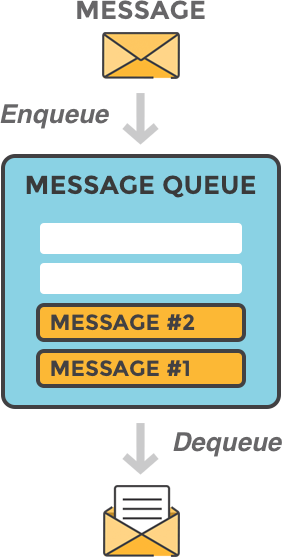
\includegraphics[width=\linewidth]{img/queue.png}
            \end{center}
        \end{column}
        \hfill
        \begin{column}{.72\linewidth}
            \begin{itemize}
                \item \alert{mono-directional}, like byte streams
                %
                \begin{itemize}
                    \item two operations: enqueue \& dequeue
                \end{itemize}

                \smallskip

                \item carrying discrete \alert{messages}, like RPC
                %
                \begin{itemize}
                    \item serialized as byte chunks
                \end{itemize}

                \smallskip

                \item commonly \alert{buffered} \& unlimited
                %
                \begin{itemize}
                    \item to support \alert{time-uncoupling}
                \end{itemize}

                \smallskip

                \item commonly, \alert{non-blocking}

                \smallskip

                \item commonly backed by ad-hoc \alert{protocols}
                %
                \begin{itemize}
                    \item[eg] AMQT, MQTT, etc.
                \end{itemize}
            \end{itemize}
        \end{column}
    \end{columns}


\end{frame}

\section{Exercises}

\subsection{First Exercise}

\startExercise

\begin{frame}[allowframebreaks]
	\frametitle{Exercise \currentExercise{} -- First Exercise}

	\begin{block}{Repository}\centering
		\url{\labRepo}
	\end{block}

	\bigskip

	Activity:
	%
	\medskip
	%
	\begin{enumerate}
		\item Have a look to the provided code

		\medskip

		\item Read the \texttt{README.md} file to figure out what to do

		\framebreak

		\item[!] Solutions which do not pass the tests are not correct
		%
		\begin{itemize}
			\item tests are provided as Bash scripts, for *nix systems
		\end{itemize}

		\medskip

		\item Push your solution on GitLab, \alert{even if incomplete}
		%
		\begin{itemize}
			\item use the \texttt{submissions/\alert{name.surnameN}} branch
			\item tests are automatically run upon push: consider it a feedback
		\end{itemize}

	\end{enumerate}

\end{frame}

%===============================================================================
\section*{}
%===============================================================================
\frame{\titlepage}

%===============================================================================
%\section*{\bibname}
%===============================================================================

%\setbeamertemplate{page number in head/foot}{}
%\\\\\\\\\\\\\\\\\\\\\
%\begin{frame}[t,allowframebreaks,noframenumbering]\frametitle{\refname}
%    \tiny
%    \bibliographystyle{plain}
%    \bibliography{sd-lab-queues}
%\end{frame}
%\\\\\\\\\\\\\\\\\\\\\

%%%%%%%%%%%%%%%%%%%%%%%%%%%%%%%%%%%%%%%%%%%%%%%%%%%%%%%%%%%%%%%%%%%%%%%%%%%%%%%
\end{document}
%%%%%%%%%%%%%%%%%%%%%%%%%%%%%%%%%%%%%%%%%%%%%%%%%%%%%%%%%%%%%%%%%%%%%%%%%%%%%%%%

